\documentclass[a4paper, 11pt, compsoc]{IEEEtran}

\usepackage{amsmath}
\usepackage{physics}
\usepackage{hyperref}
\usepackage{cleveref}
\hypersetup{
	colorlinks = true,
	linkcolor = blue,
	filecolor = blue,
	citecolor = black,
	urlcolor = cyan,
}
\crefname{appsec}{Appendix}{Appendices}

\usepackage{graphicx}
\usepackage[section]{placeins}
\usepackage{bookmark}
\usepackage{gensymb}


%for code(MATLAB in particular)
\usepackage{listings}
\usepackage{color} %red, green, blue, yellow, cyan, magenta, black, white
\definecolor{mygreen}{RGB}{28,172,0} % color values Red, Green, Blue
\definecolor{mylilas}{RGB}{170,55,241}

\lstset{
    language=Matlab,%
    %basicstyle=\color{red},
    breaklines=true,%
    morekeywords={matlab2tikz},
    keywordstyle=\color{blue},%
    morekeywords=[2]{1}, 
    keywordstyle=[2]{\color{black}},
    identifierstyle=\color{black},%
    stringstyle=\color{mylilas},
    commentstyle=\color{mygreen},%
    showstringspaces=false,%without this there will be a symbol in the places where there is a space
    numbers=left,%
    numberstyle={\tiny \color{black}},% size of the numbers
    numbersep=7pt, % this defines how far the numbers are from the text
    emph=[1]{for,end,break},
    emphstyle=[1]\color{red}, %some words to emphasise
    %emph=[2]{word1,word2}, emphstyle=[2]{style},
}


\graphicspath{{./pictures/}}

\title{ECEN315 - Compensating a Propeller Driven Pendulum }
\author{Joshua Benfell - 300433229}

\IEEEtitleabstractindextext{
	\begin{abstract}
		This report expands on the mathematical model of a propeller driven pendulum and aims to compensate a practical model that varies from this derived model. Various compensators were trialed before settling on the PID compensators. Once tuned the compensator was able to remove the steady state error, overshoot and oscillation and reduce the settling time down to less than 1 second from an expected 6 seconds.
    \end{abstract}
}


\begin{document}
    \maketitle
    \IEEEdisplaynontitleabstractindextext

    \section{Introduction}\label{sec:intro}
		In the previous report the open loop transfer function was derived for a propeller driven pendulum. The response of the system was stable with oscillations making it unideal for practical use. To improve the system, a compensator will be designed for it to speed up the systems response and make it less oscillatory. To do this, a variety of compensators will be modelled using the simulink package to gain a better understanding of the function and benefits of them. Finally a PID compensator will be implemented with that reduces the settling time of the system at least threefold down from 6 seconds.
	\section{Background}\label{sec:bg}
		This paper will be investigating various closed loop compensators, building up to a PID compensator. A PID compensator aims to improve the response of a system, by increasing speed and stability, removing steady state error, reducing overshoot and improving the response to disturbances \cite{elprocus}. However, it is possible to reduce the compensator to include less blocks, such as PI and PD, which this paper will be covering to gain a better understanding of what the individual components contribute to the response.
		\par
		A common topic talked about in this report is the concept of stability and when a system becomes unstable. This behavior is predictable through the use of a few tools, notably for this report, root locus and Bode plots. From the root locus, stability for a certain feedback gain is able to be discerned from when the root locus paths cross over the imaginary axis and become positive. With Bode plots, stability can be determined from the phase margin. This value is found by reading the phase shift when the gain goes from positive gain to negative gain (in dB). If the phase margin is greater than -180 degrees then the system is stable. In both of these cases, the negative feedback normally employed in these closed loop systems becomes positive feedback which causes the system to grow without bounds.
	\section{Simulink Model}\label{sec:model}
		\begin{figure}[!ht]
			\centering
			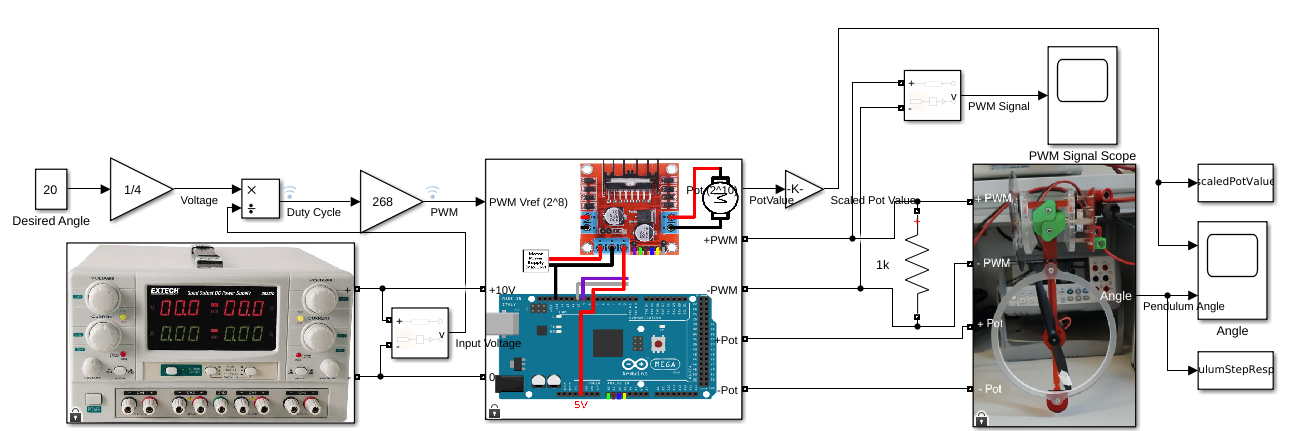
\includegraphics[width=\columnwidth]{lab4System.png}
			\caption{Calibrated Open Loop System}
			\label{fig:baseSystem}
		\end{figure}
		In the last report, the transfer function of our system was derived, however, the derived system is not always an accurate representation of how the actual system will behave. To imitate this dissonant behavior, a slightly different system will be used in the simulink models. The system used in this report (shown in \Cref{fig:baseSystem}, where it is fully calibrated.), takes a PWM reference and then outputs the resultant angular displacement. However, it is desirable that the input units are the same as the output units, so the system needs to be calibrated.
		\par
		There are 3 main calibration stages on the input sides:
		\begin{itemize}
			\item Converting the desired angular displacement into the required applied voltage.
			\item Converting that voltage into a duty cycle
			\item Converting that duty cycle into the PWM value the arduino should output to the motor
		\end{itemize}
		To calibrate these values first start with the angle. By applying a voltage over the pendulum motor an angular displacement can be generated. By applying different voltages, a relationship can be determined between the voltage and the angle. For this system it was found that the voltage required is 4 times less than the desired angle (\Cref{app:calibration}).
		\par
		\begin{figure}[!ht]
			\centering
			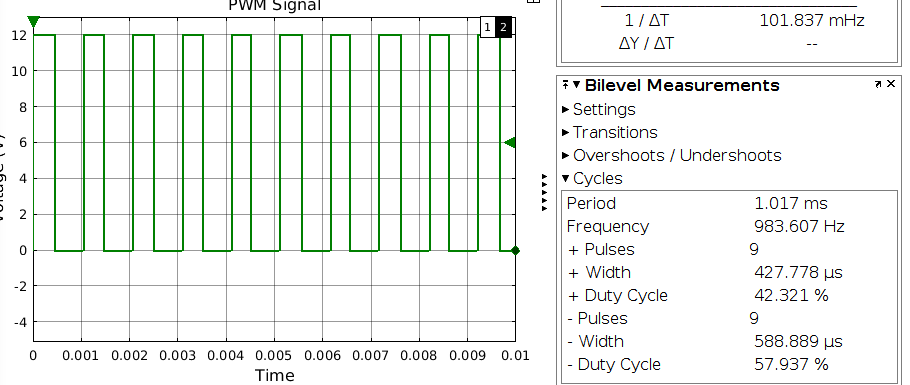
\includegraphics[width=\columnwidth]{dutyCycleSignal.png}
			\caption{Signal Generated by the Arduino}
			\label{fig:signal}
		\end{figure}
		The next constant to determine is the conversion between voltage and a duty cycle. To do this, the system incorporates the arduino to control the effective voltage applied to the motor. A series of PWM values are input into the arduino and the resultant signal will be read across a $1k\Omega$ load, were the duty cycle can be measured (\Cref{fig:signal}). Plotting the relationship between duty cycle and PWM and voltage and duty cycle result in the constants 2.68 and 1/12 respectively (\Cref{app:calibration}); this second constant is 1 over the source voltage. A factor of 100 needs to be added in somewhere along this cascaded chain as the duty cycle is shown as a percentage not a proportion.
		\par
		With the above constants computed, the pendulum will now rise to the desired angle. There is one final constant to compute, and that is the constant to convert the analog potentiometer value into an angle so that the angle can be read for later application; practically the arduino is unable to read the angular displacement without a component such as a potentiometer. To calibrate this constant, the potentiometers value is plotted against the resulting angle; the constant that converts the ADC value to an angle is 1/25 (\Cref{app:calibration}).
		\begin{figure}[!ht]
			\centering
			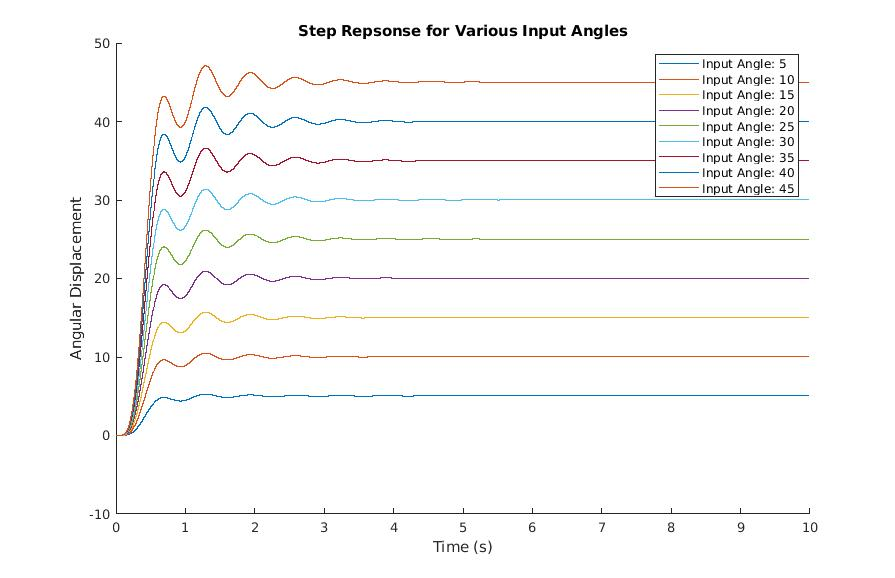
\includegraphics[width=\columnwidth]{lab4Input.jpg}
			\caption{System Response to various desired angles}
			\label{fig:lab4Output}
		\end{figure}
		\begin{figure}[!ht]
			\centering
			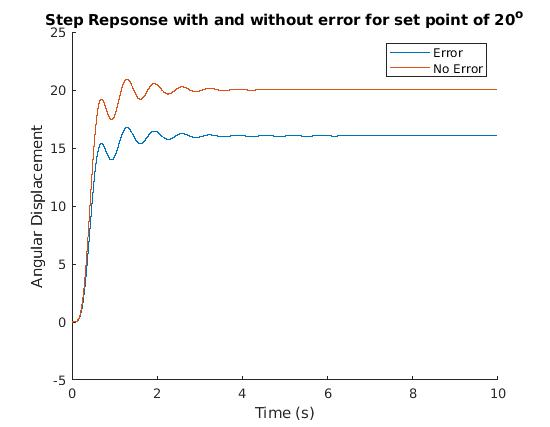
\includegraphics[width=\columnwidth]{lab4Error.jpg}
			\caption{System Response with and without a simulated Error}
			\label{fig:lab4Error}
		\end{figure}
		\begin{table}
			\centering			
			\begin{tabular}{l|r}
				Parameter         & \multicolumn{1}{l}{Value} \\ \hline
				Rise Time (s)     & 0.3401                    \\
				Settling Time (s) & 2.006                     \\
				OS\%              & 4.5631                    \\
				Peak Time (s)     & 1.2911                   
				\end{tabular}
			\caption{Transient Response Data for the calibrated System}
			\label{tab:transientResLab4}
		\end{table}
		Finally, the calibrated system needs to be tested to confirm that it reaches the desired input. \Cref{fig:lab4Output} shows the output to various desired inputs, and it can be seen that the system has zero steady state error for all the inputs. The transient characteristics are presented in \Cref{tab:transientResLab4}. From these measurements it can be seen that the system has a quick response being able to settle in 2 seconds.
		\par
		However, not all systems are perfect and as such we are able to simulate an error (\Cref{fig:lab4Error}). The relation between the error and the steady state value for the system with simulated error is that the error is $0.2 \times \text{steady state value}$, so to account for this, a gain of 1.25 is applied to the input angle (as the steady state value will be 0.8 the input angle) \Cref{app:calibration}. This is not an ideal solution to deal with the error as this requires a different gain value if a different error exist, and this may not be linear, it also limits the range of angles that the pendulum can settle on as the higher input angle will top off the PWM signal sooner. The simulated error in the system does not appear to effect the transient response of the system, where in a physical system, error in the system could potentially do this. This could be in the form of making it more oscillatory or lengthening the time it takes to settle. So it should be clear that this open loop control is unsuitable for a realistic system. However, by calibrating it, it is now possible to use the system more intuitively from having the input and outputs match in units. This makes compensator design easier.
	\section{Compensators}\label{sec:comp}
		To account for some of the issues mentioned in \Cref{sec:model} around open loop systems the use of closed loop compensators will be employed. Currently the open loop plant $G(s) = \frac{N(s)}{D(s)}$ (\Cref{app:oltf}) with a given compensator $K(s)$, takes the form $K(s) G(s)$. By closing the loop with negative feedback it will take the form in \Cref{eq:cltf,app:cltf}.
		\begin{equation}
			\label{eq:cltf}
			\begin{split}
				\frac{K(s)G(s)}{1 + K(s)G(s)} & = \frac{K(s)\frac{N(s)}{D(s)}}{1 + K(s)\frac{N(s)}{D(s)}} \\
				& = \frac{K(s)N(s)}{D(s) + K(s)N(s)}\\
			\end{split}
		\end{equation}
		\par
		Which shows that by adding a compensator in negative feedback, the numerator of the transfer function gets scaled by the compensator, and then added to the denominator. 
		\subsection{Proportional}\label{sec:p}
			The proportional compensator is one which takes the form of a constant, $K(s) = K_p$. To establish a starting value for $K_P$, the previously determined transfer function can be used in a root locus plot, however will need to be compensated to convert the function it to $\frac{\Theta}{\Theta}$ instead of the current $\frac{\Theta}{V}$. To convert this function to be the transfer between two angles in degrees, it gets multiplied by $0.057$ to convert the input angle into a voltage and $\frac{180}{\pi}$ to convert the output angle in radians, into one in degrees.
			\begin{figure}[!ht]
				\centering
				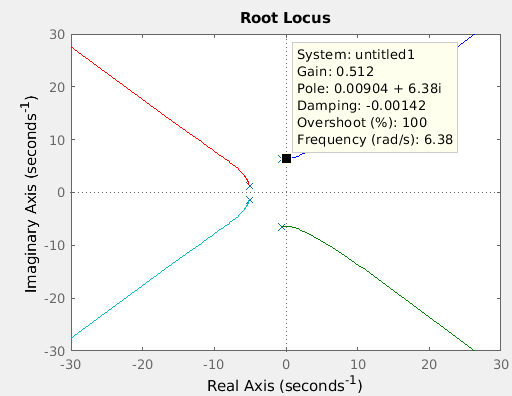
\includegraphics[width=\columnwidth]{lab5RLocus.png}
				\caption{Root Locus of the Calibrated Matlab Transfer Function}
				\label{fig:lab5RLocus}
			\end{figure}
			\par
			From \Cref{fig:lab5RLocus} it can be seen that the gain value that causes the simulated matlab transfer function to go unstable is approximately $K_P > 0.5$. By starting the proportional compensator at this value, the simulink model can be expected to have undamped oscillation, then the value can be lowered until the desired outcome is reached. However, due to the fact that the two models differ slightly, it turns out that the observed gain value in the root locus is much lower than the gain value that causes the system to be unstable as seen in \Cref{fig:lab5KP}.
			\begin{figure}[!ht]
				\centering
				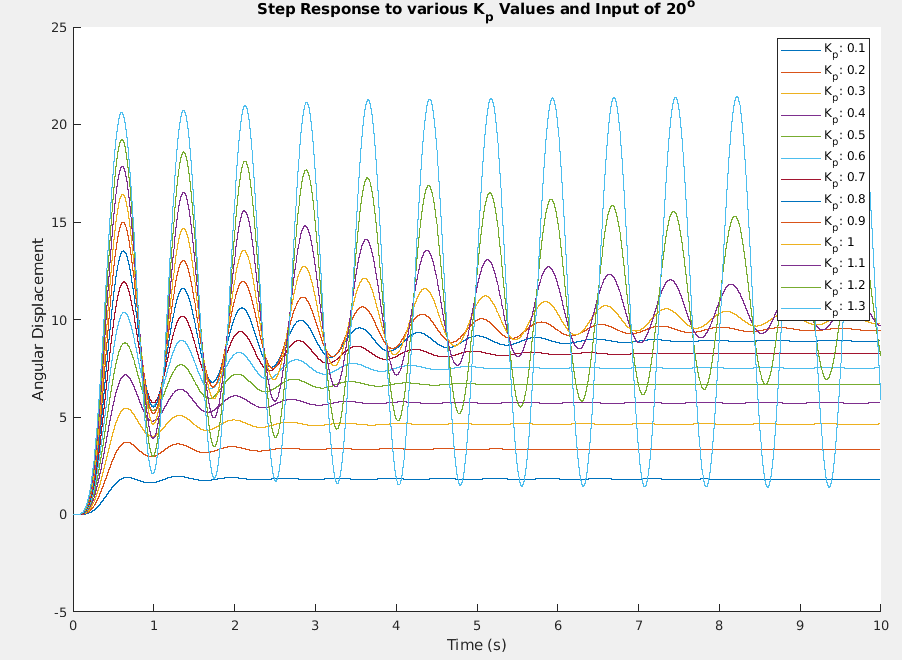
\includegraphics[width=\columnwidth]{lab5KP.png}
				\caption{Response to a Proportional Compensator with varying $K_P$}
				\label{fig:lab5KP}
			\end{figure}
			\begin{table}
				\label{tab:lab5KPRT}
				\centering
				\begin{tabular}{r|r}
					$K_P$ & Rise Time (s)\\
					\hline
					0.1 & 0.296610531126288\\
					0.2 & 0.275038044405800\\
					0.3 & 0.257477359386261\\
					0.4 & 0.242452588954751\\
					0.5 & 0.230629632201802\\
					0.6 & 0.221720597290433\\
					0.7 & 0.213498804733117\\
					0.8 & 0.206000853194294\\
					0.9 & 0.199620596553673\\
					1.0 & 0.192416472953142\\
					1.1 & 0.181419416207832\\
					1.2 & 0.160047304029543\\
					1.3 & 0.135340118169653\\
				\end{tabular}
				\caption{Rise Times for \Cref{fig:lab5KP}}
			\end{table}
			\Cref{fig:lab5KP} shows the response to different $K_P$ values and it can be seen that $K_P = 0.5$ does not cause the system to have near undamped oscillation like the previous model would suggest. In fact, this doesn't happen until $K_P = 1.3$ where it can be seen that the system has started reaching the limits of it's growth, indicating that without these limits it would be an unstable system. One of the consequences of the proportional compensator on this system is that there is an increased steady state error for lower values of $K_P$. Referring back to \Cref{eq:cltf}, the cause of this can be seen to be the $s^0$ term being larger on the bottom than the top and being much larger for lower values of $K_P$ as the term is not scaled in the denominator.
			\par
			To reduce the steady state error, just increase the $K_P$ value. However, this has it's own consequences. As is visible in \Cref{fig:lab5KP}, as $K_P$ is increased, so is the oscillation in the response, till eventually it becomes unstable. As a result of the instability, it is not possible to make $K_P$ large enough to remove the steady state error before this happens, meaning something else is needed. A positive consequence of increasing $K_P$ is that the system responds faster, evident by the rise times shown in \Cref{tab:lab5KPRT}. Finally, as shown in \Cref{fig:lab5Error} it can be seen that a proportional compensator on it's own is unable to effectively remove errors in the system, to match the original non-simulated error response.
			\begin{figure}[!ht]
				\centering
				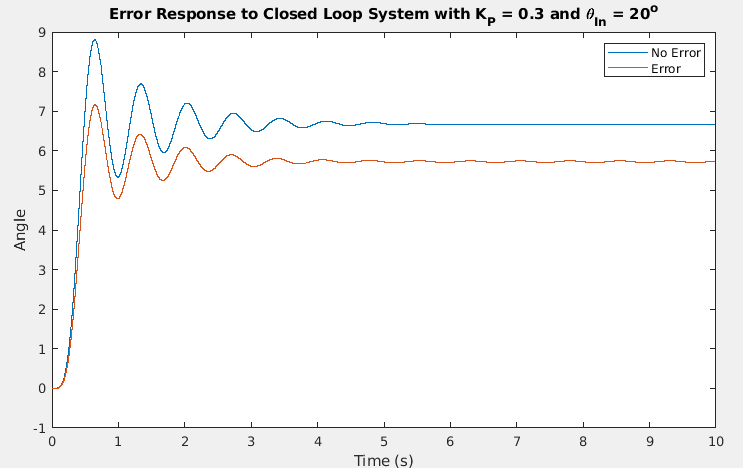
\includegraphics[width=\columnwidth]{lab5Error.png}
				\caption{Response with and Without Simulated Error}
				\label{fig:lab5Error}
			\end{figure}
			\par
			From \Cref{fig:lab5KP}, it is evident that the system can and will go unstable under the right conditions. If this were a physical system this is a hazard that is quite threatening to those around the system. So as a safety measure for if this simulation gets used to control a physical system, a software switch has been added to easily turn the system off. As such the final system with an incorporated P compensator looks like \Cref{fig:lab5Sys}.

			\begin{figure}[!ht]
				\centering
				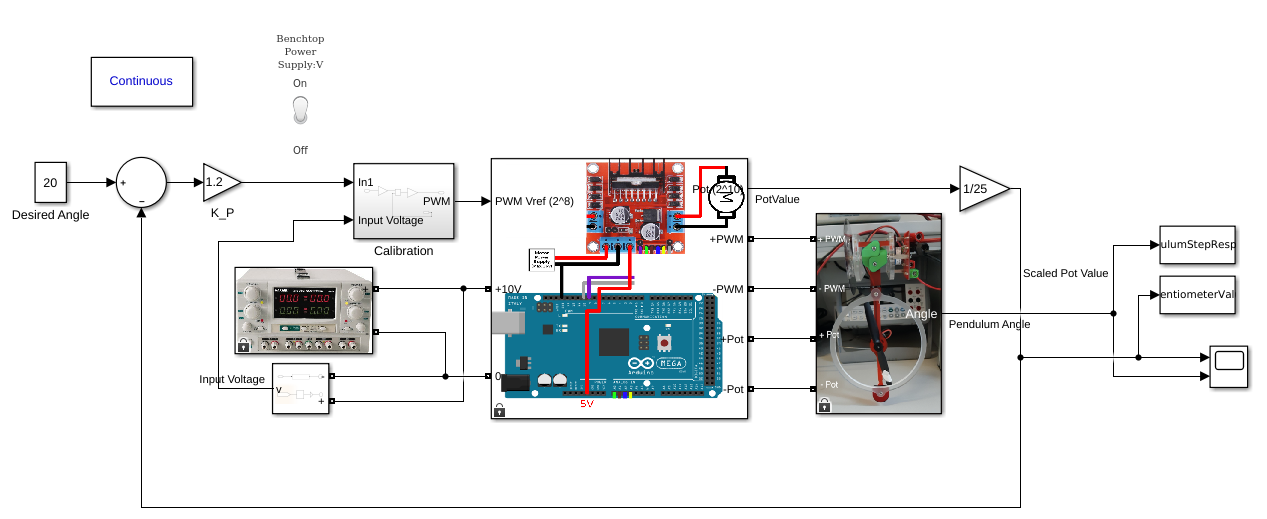
\includegraphics[width=\columnwidth]{lab5Sys.png}
				\caption{System with a Closed Loop Proportional Compensator Incorporated}
				\label{fig:lab5Sys}
			\end{figure}

		\subsection{PI}\label{sec:pi}
			The next compensator to be investigated is the proportional, integral or PI compensator. The PI controller adds an open loop pole at zero, giving infinite gain at low frequencies. Not only does it add this pole, it also adds an open loop zero to the system at $\frac{K_i}{K_p}$ (\Cref{eq:PIeq}). The addition of these roots has tugged on the root locus of the system more towards the real axis initially and effected how the gain changes the system, enough to require a higher gain before the system becomes unstable (\Cref{fig:lab6PIRlocus}). The addition of a pure integrator (making this a type 1 system) has an additional benefit in that it reduces the steady state error for step inputs to 0.
			\par
			\begin{equation}
				\label{eq:PIeq}
				\begin{split}
					K(s) & = \frac{K_i}{s} + K_p \\
						 & = \frac{K_i + K_ps}{s} \\
						 & = K_p \frac{\frac{K_i}{K_p} + s}{s}
				\end{split}
			\end{equation}

			\begin{figure}[!ht]
				\centering
				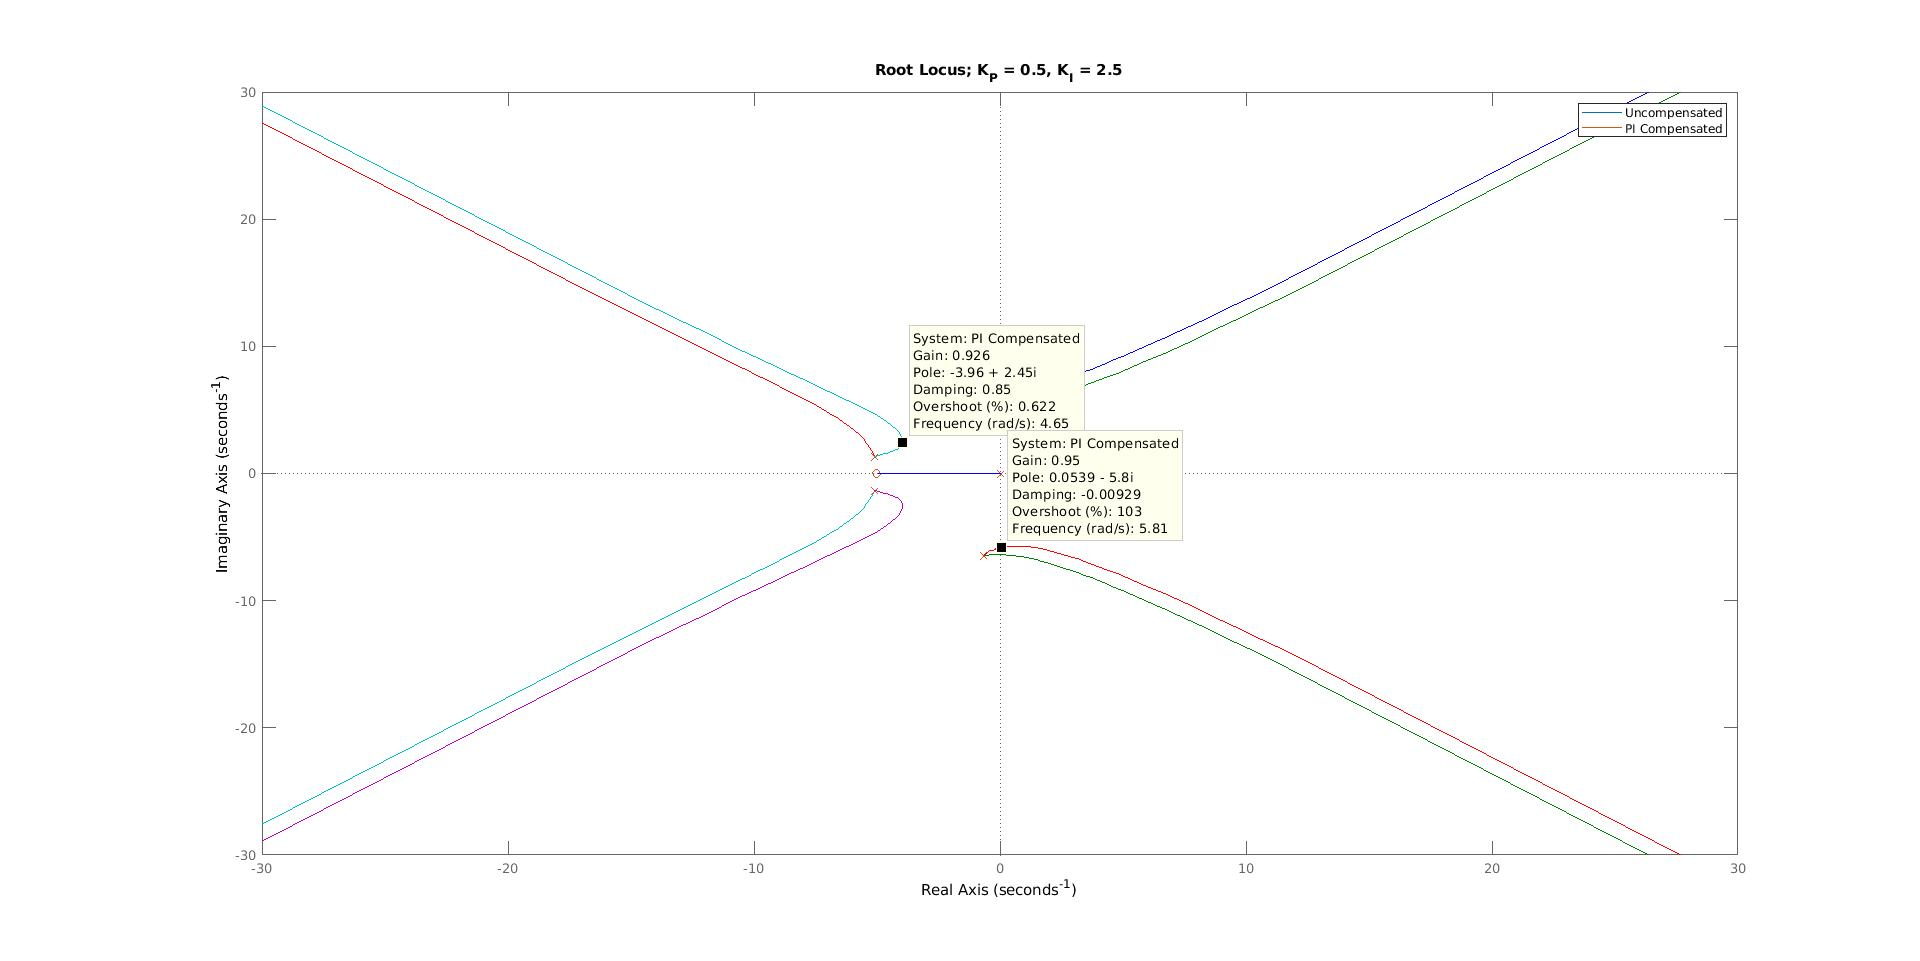
\includegraphics[width=\columnwidth]{lab6PIRlocus.jpg}
				\caption{Root Locus of the Matlab System with and Without a PI compensator}
				\label{fig:lab6PIRlocus}
			\end{figure}

			\begin{figure}[!ht]
				\centering
				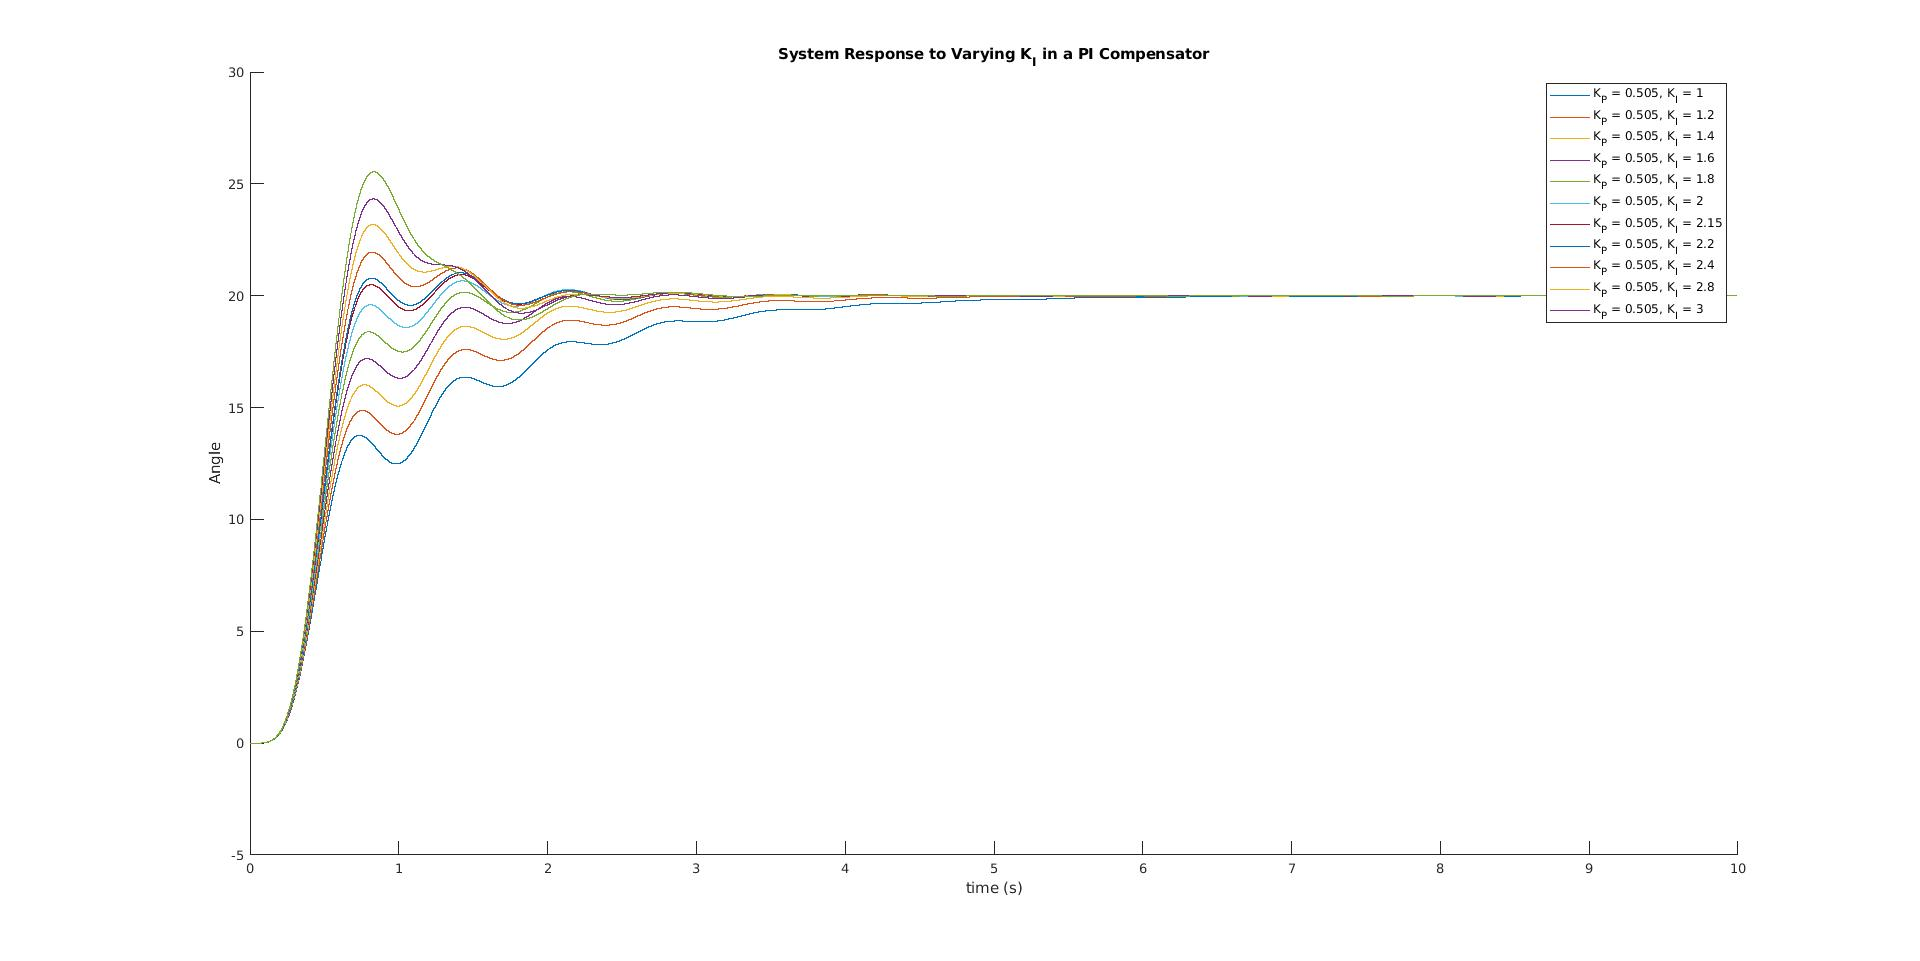
\includegraphics[width=\columnwidth]{changeK_iInPICompensator.jpg}
				\caption{Changing the Simulink Systems $K_i$ for $K_p = 0.505$}
				\label{fig:lab6PI_Ki_Change}
			\end{figure}

			\begin{figure}[!ht]
				\centering
				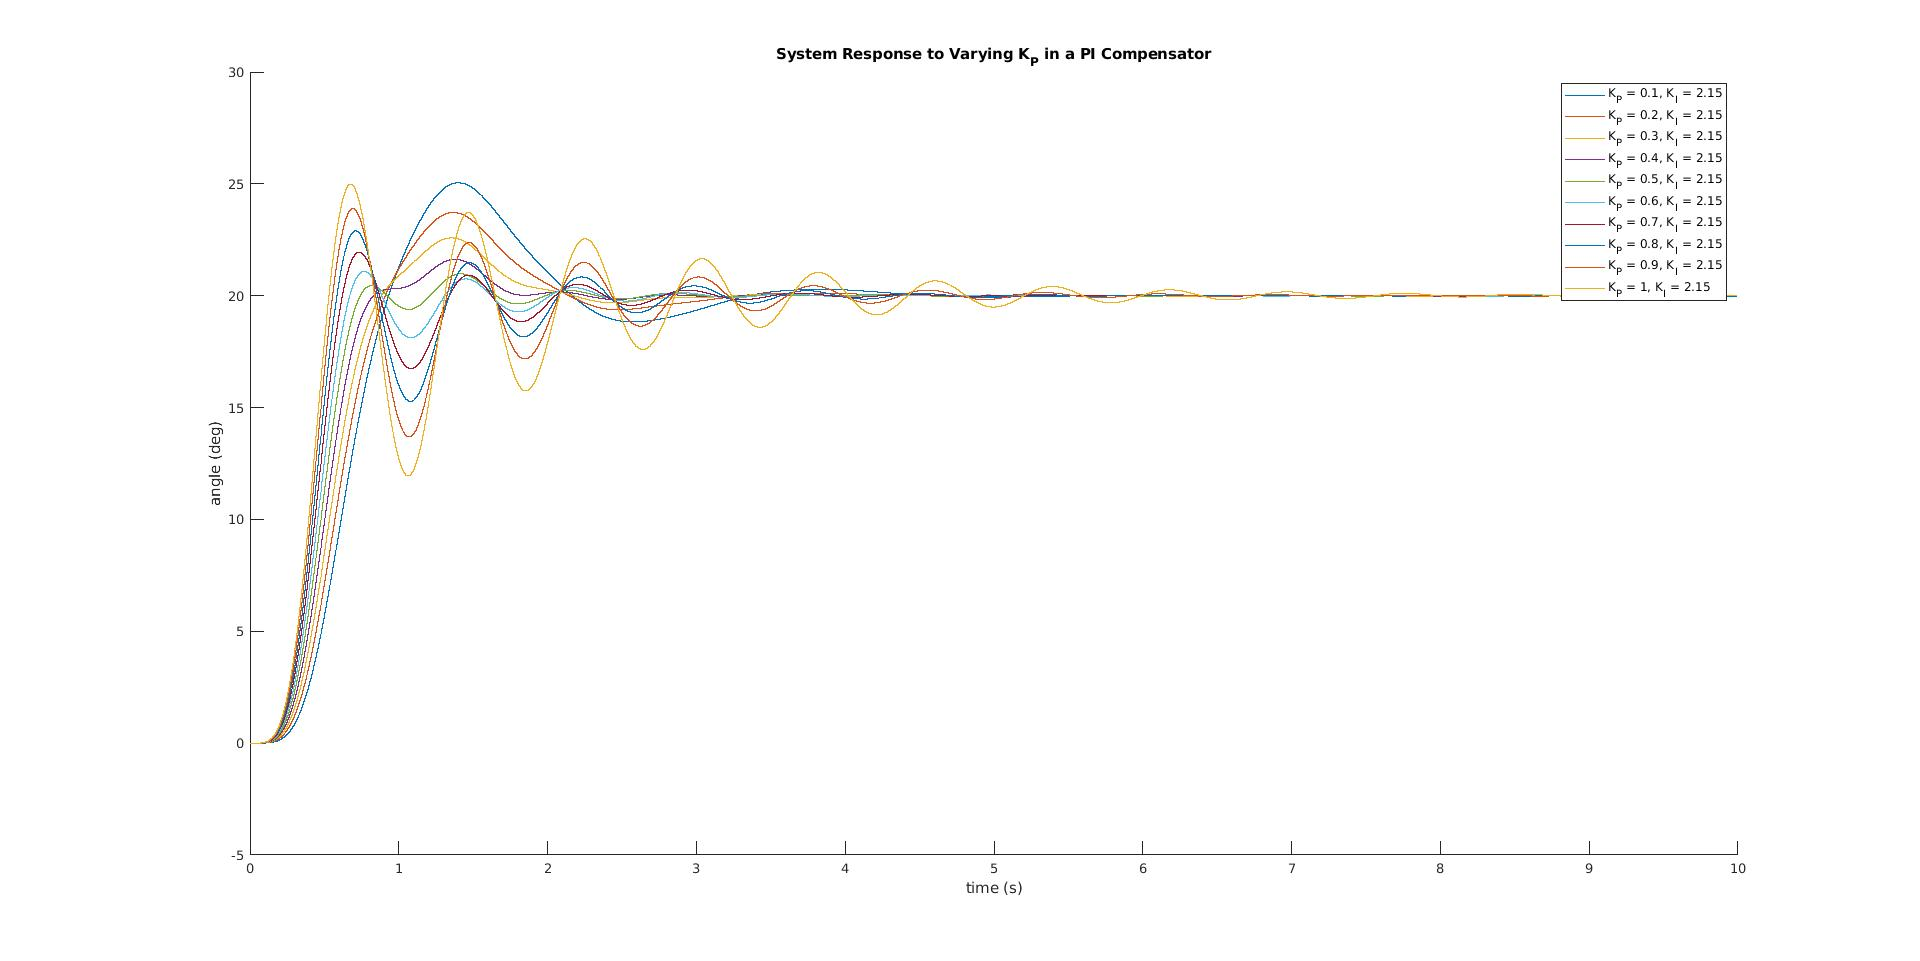
\includegraphics[width=\columnwidth]{changeK_pInPICompensator.jpg}
				\caption{Changing the Simulink Systems $K_p$ for $K_i = 2.15$}
				\label{fig:lab6PI_Kp_Change}
			\end{figure}
			This compensator will first be implemented with $K_P = 0.505$ which is the value determined from \Cref{fig:lab5RLocus}. From then $K_i$ was varied to gain an understanding of what the parameter did to the behavior of the system. From \Cref{fig:lab6PI_Ki_Change} it can be seen that just adding the PI controller fully removes the steady state error from the system. \Cref{fig:lab6PI_Ki_Change} also shows that increasing $K_i$ reduces the time it takes for the system to reach a value close to the target, and so long as it doesn't overshoot by a lot, reduce the time it takes to settle. This occurs as the compensator integrates more with higher $K_i$ such that it responds to further away error better, however, as is evident in \Cref{fig:lab6PI_Ki_Change}, if it integrates too much then it will overshoot more than is desired, as the ideal response is a non-oscillatory rise to the final value. 
			\par
			\begin{figure}[!ht]
				\centering
				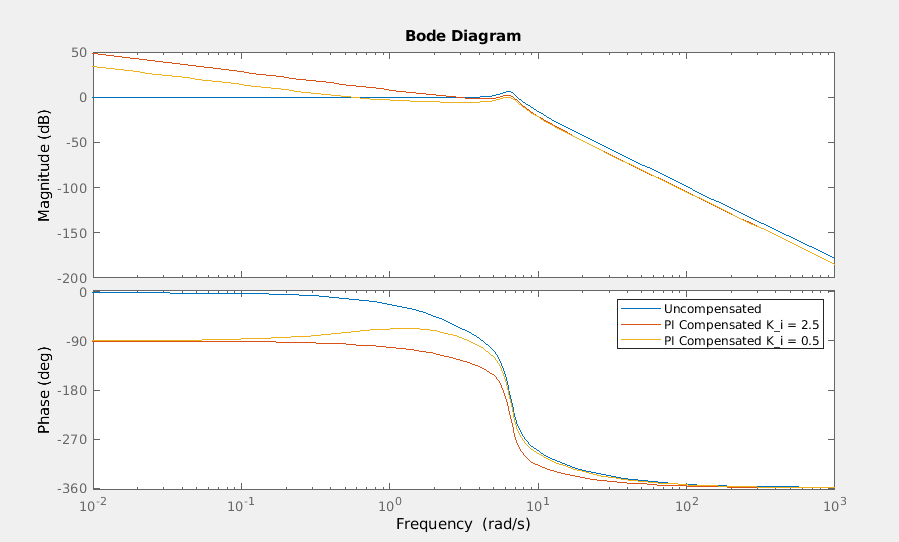
\includegraphics[width=\columnwidth]{PIBode.png}
				\caption{Bode Plot for a PI compensator}
				\label{fig:pibode}
			\end{figure}
			Typically, it is desired that the zero created by the PI controller is close to zero. This is the case because it has less effect on the phase after the zero which improves or doesn't effect the phase margin. This helps ensure that the system remains stable or becomes stable. This effect can be seen in \Cref{fig:pibode} where the PI controllers have shifted the unity crossing point to a frequency where the phase is more significantly bigger than -180 degrees, which provides more leeway for gain as well as mentioned before. However, as shown by \Cref{fig:lab6PI_Ki_Change}, this does not always produce the most desirable behavior as it can be slow.
			\par
			The other parameter to vary is $K_p$, due to the way the compensator is implemented (\Cref{fig:piSys}), changing $K_p$ also shifts the zero around. From \Cref{fig:lab6PI_Kp_Change}, it can be seen that the effect $K_p$ has on the response is it speeds it up but at the cost of making it more oscillatory. Looking at the bode plot (\Cref{fig:PIKPBode}), it can be seen that the lower $K_p$ value has the zero place further away from the integrator at $21.5 \text{rad/s}$ which causes the phase shift to happen later than the $K_p = 0.5$ system nearly causing a case of instability. So this indicates that if lower $K_p$ values are required, to reduce the oscillations they introduce, lower $K_i$ values should also be used to reduce the risk of instability by placing the zero closer to zero. 
			\begin{figure}[!ht]
				\centering
				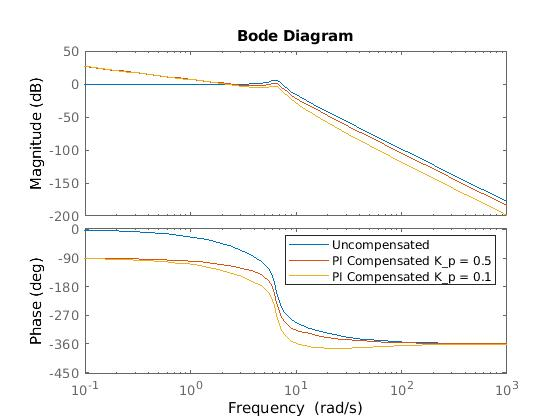
\includegraphics[width=\columnwidth]{PI_KP_Bode.jpg}
				\caption{Bode Plot for a PI Compensator with Changing $K_p$}
				\label{fig:PIKPBode}
			\end{figure}
			\par
			From the tuning done with the PI compensator, it was found that $K_p = 0.505$ (the matlab transfer functions crossing point) and $K_i = 2.15$ provided a suitable response with a $2 s$ settling time and $4\%$ overshoot while also removing the steady state error, even with a simulated error (\Cref{fig:PI_Error}). 
			\begin{figure}[!ht]
				\centering
				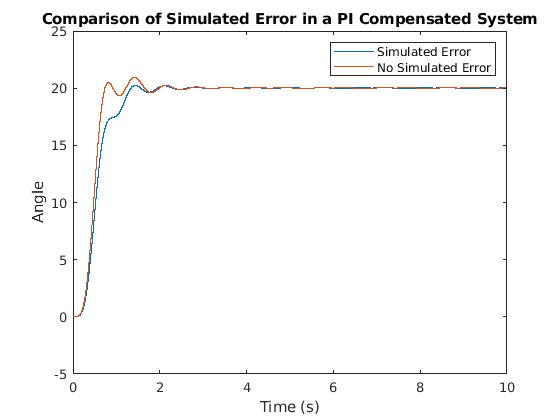
\includegraphics[width=\columnwidth]{PI_Error.jpg}
				\caption{Comparison Error Rejection for PI Compensated System with and without a Simulated Error}
				\label{fig:PI_Error}
			\end{figure}

			\begin{figure}[!ht]
				\centering
				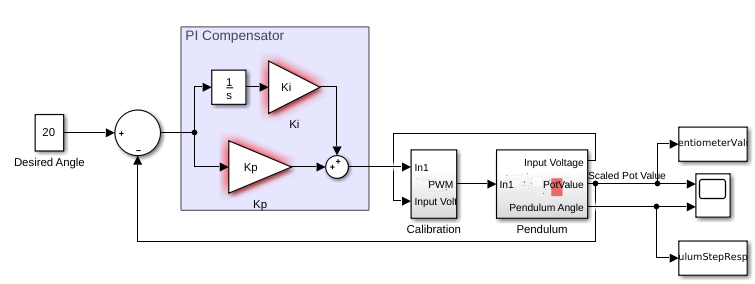
\includegraphics[width=\columnwidth]{piSys.png}
				\caption{Implementation of a PI Compensator in Simulink}
				\label{fig:piSys}
			\end{figure}

		\subsection{PD}\label{sec:pd}
			The proportional, derivative compensator, PD, is a compensator that has infinite gain at high frequencies and introduces an open loop zero into the system at $\sigma = -\frac{K_p}{K_d}$ (\Cref{eq:pdeq}). From \Cref{fig:lab6PDrl} it can be seen that the effect of this zero redirects the root locus to the real axis making some of the poles less oscillatory as the gain is increased. \Cref{fig:lab6PDBode} shows that the zero also effects the phase margin. It shifts the unity crossing point to the right which will typically make the crossing point happen at a location with a phase shift closer or beyond -180 degrees, indicating that the PD controller will be very sensitive to instability. Additionally it also adds a phase shift of +90 degrees, which can help the phase not drop off as fast or improve the gain margin potentially. However, it appears that the PD controller will be sensitive and the immediate benefits will not be seen here.
			\par
			\begin{equation}
				\label{eq:pdeq}
				\begin{split}
					K(s) & = K_ds + K_p\\
						 & = K_d(s + \frac{K_p}{K_d})\\
				\end{split}
			\end{equation}
			\begin{figure}[!ht]
				\centering
				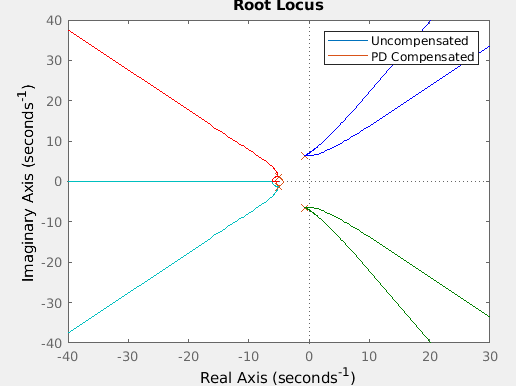
\includegraphics[width=\columnwidth]{lab6PDrl.png}
				\caption{Root Locus of a PD Compensated System with $K_d = 0.1$ and $K_p = 0.5$}
				\label{fig:lab6PDrl}
			\end{figure}

			\begin{figure}[!ht]
				\centering
				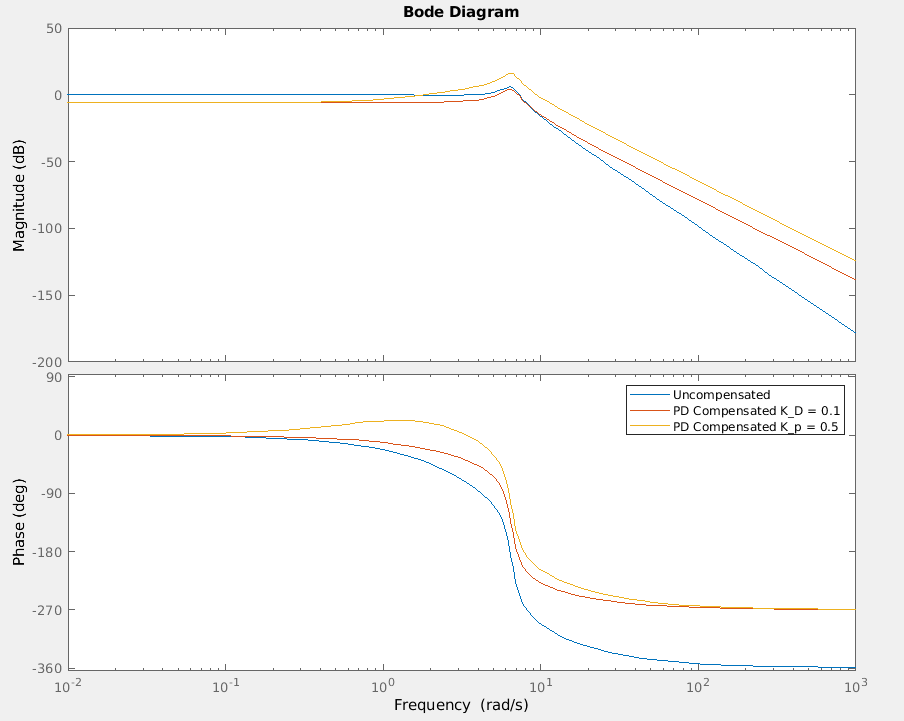
\includegraphics[width=\columnwidth]{lab6PDBode.png}
				\caption{Bode Plot of PD Compensated Systems}
				\label{fig:lab6PDBode}
			\end{figure}

			\begin{figure}[!ht]
				\centering
				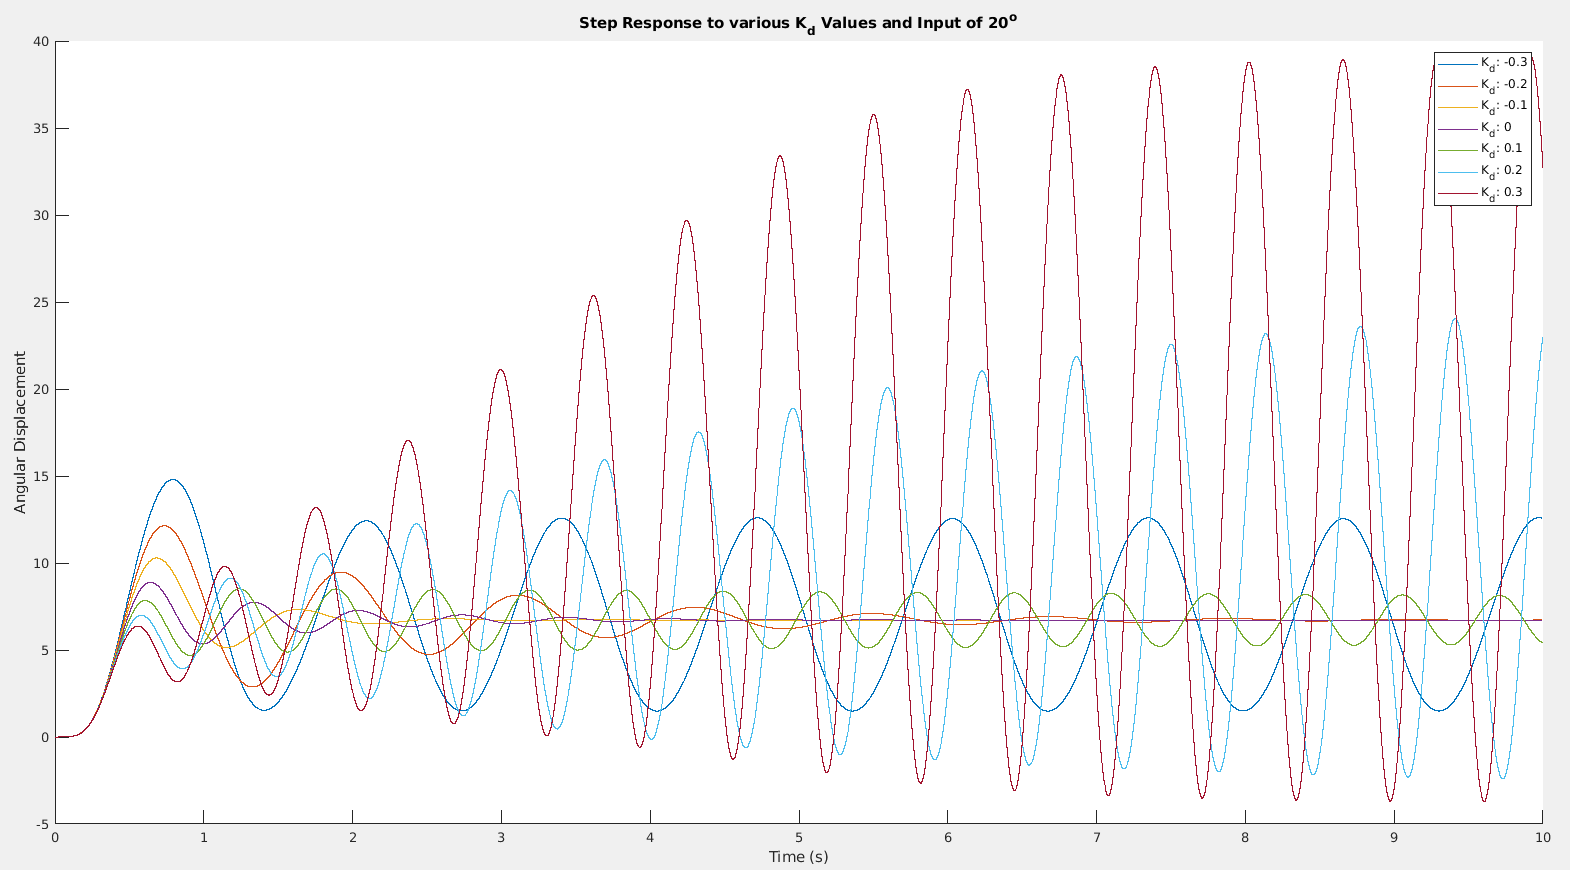
\includegraphics[width=\columnwidth]{lab6PDStep.png}
				\caption{Step Response for Various $K_d$ values in the Simulink Model}
				\label{fig:lab6PDStep}
			\end{figure}

			Running some simulations with the Simulink model, \Cref{fig:lab6PDStep} shows that there is a very small range of usable values and that positive $K_d$ values will add oscillations to the system and make it unstable sooner than a negative value. $K_d = -0.1$ seems to be the best value of those simulated here as it removes a lot of the oscillations in the system, however, it does increase the overshoot. This makes sense as the zero close to the dominant poles would redirect them to move closer to the real axis, reducing oscillations. So long as your gain value is low enough to not make the system unstable, this will work for the system being used. One of the downsides of the standalone PD compensator is that it has a relatively large steady state error, so to remedy this, the P, I and D elements discussed so far will be combined into one compensator. 

		\subsection{PID}\label{sec:pid}
			\subsubsection{Putting it Together}\label{sec:pidtune}
				Now that PI and PD compensators have been investigated and a better understanding of how the values effect the pendulum system has been established, it is time to combine all the elements into a PID compensator. The requirements for this compensator are that it has overshoot and undershoot no greater than 2\% and has a settling time less than 2 seconds, which is a threefold increase on the standard settling time of 6 seconds. The compensator takes the form from \Cref{eq:pideq}, which introduces two open loop zeros and makes it a type 1 system. 
				\par
				\begin{equation}
					\label{eq:pideq}
					\begin{split}
						K(s) & = K_p + \frac{K_i}{s} + K_ds\\
							 & = \frac{K_ds^2 + K_ps + K_i}{s}\\
							 & = K_d\frac{s^2 +\frac{K_p}{K_d}s + \frac{K_i}{K_d}}{s}
					\end{split}
				\end{equation}
				To compensate the simulink model, the initial values will be those that have been shown beforehand in \Cref{sec:pi,sec:pd}, $K_p = 0.505$, $K_i = 2.18$ and $K_d = -0.1$. \Cref{fig:lab6pid1} shows the response to these values and it can be seen that this is more oscillatory than desired, however, it does have a rise time of 300ms which is a good indication the second requirement can be met. By lowering the $K_p$ value, it should be possible to remove most of the oscillation. Some of it will be from the integral component, so if $K_p$ is too small, $K_i$ will also need to be lowered to move the zero further away, so when it's in the closed loop system it has less effect. However, the initial values found have been a good starting point as the main issue is oscillation, there is no steady state error and the rise time is fast enough to expect that it is possible to easily get the desired improvement. 
	
				\begin{figure}[!ht]
					\centering
					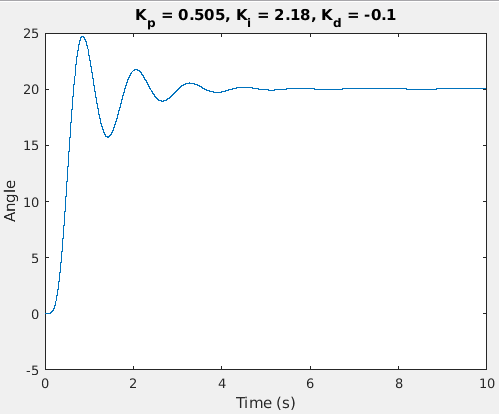
\includegraphics[width=\columnwidth]{lab6pid1.png}
					\caption{Simulink Step Response for $K_p = 0.505$, $K_i = 2.18$ and $K_d = -0.1$}
					\label{fig:lab6pid1}
				\end{figure}

				\begin{figure}[!ht]
					\centering
					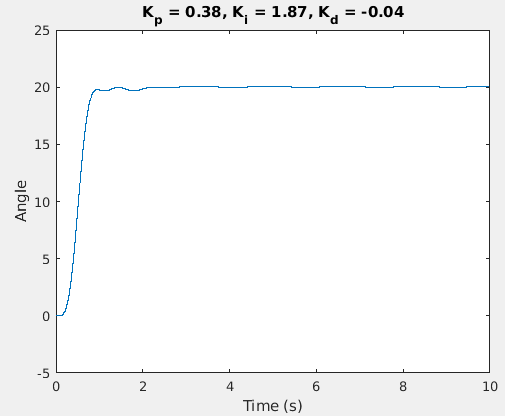
\includegraphics[width=\columnwidth]{lab6pid2.png}
					\caption{Simulink Step Response for $K_p = 0.38$, $K_i = 1.87$ and $K_d = -0.04$}
					\label{fig:lab6pid2}
				\end{figure}

				\par
				After some tuning, the values $K_p = 0.38$, $K_i = 1.87$ and $K_d = -0.04$ were found to be suitable for the system. There is 0.3\% overshoot and 2\% undershoot resulting in a settling time of 0.86s. By lowering $K_p$ and $K_p$ the zeros in the compensator were moved closer to the imaginary axis, but by lowering $K_d$, they were then moved out again. \Cref{fig:lab6pidrl} shows that this has in fact moved the zeros further away from where they were. Combining this with the matlab system (\Cref{fig:lab6pidmatlabrl}) it can be seen that the root locus tugs on the further away poles on a little bit as the integrator pole occupies the connection to the real axis zero. It then also pulls the dominant poles to the real axis well into the unstable region, however, the gain being used here keeps the poles in the stable region, but unlike the simulink system, indicate that they would still introduce some oscillatory motion. This is visible in the step response, \Cref{fig:lab6pidmatlabStep}, where there is a 50\% overshoot and a settling time of 300s. This is drastically different from the simulink model.

				\begin{figure}[!ht]
					\centering
					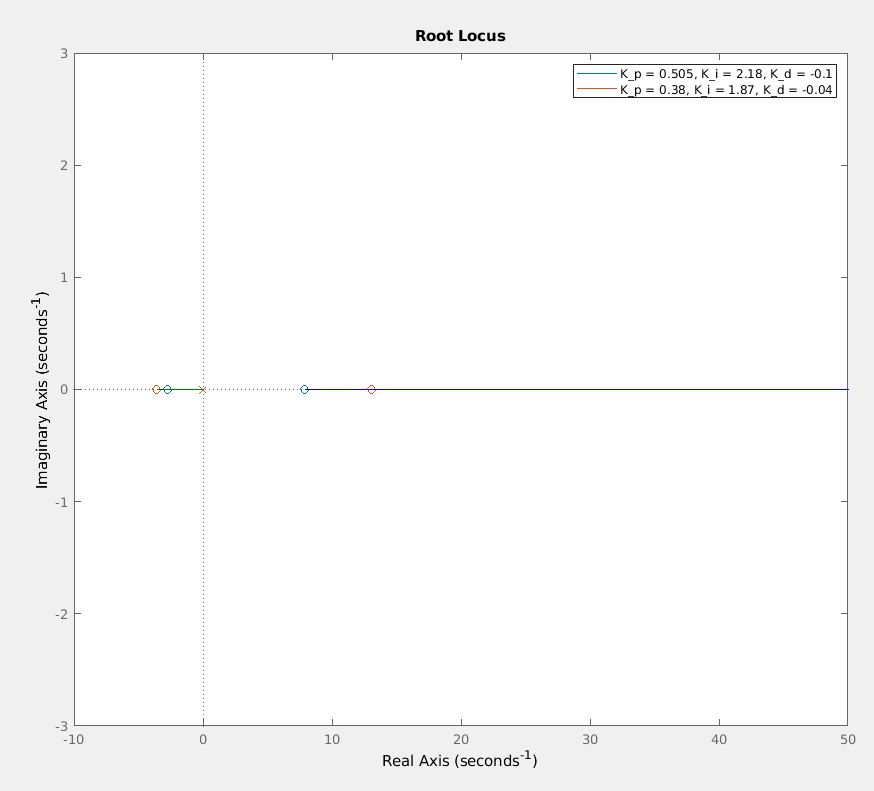
\includegraphics[width=\columnwidth]{lab6pidrl.png}
					\caption{Root Locus for the Two Compensators Tried}
					\label{fig:lab6pidrl}
				\end{figure}

				\begin{figure}[!ht]
					\centering
					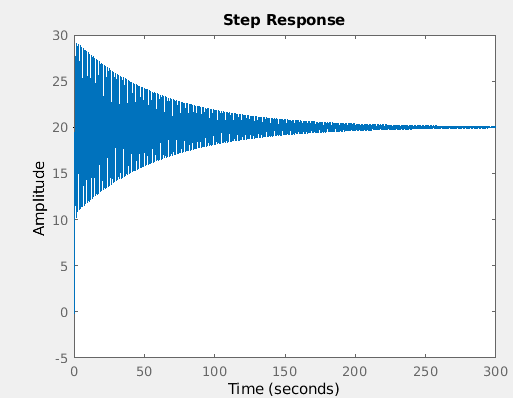
\includegraphics[width=\columnwidth]{lab6pidmatlabStep.png}
					\caption{Matlab Step Response for $K_p = 0.38$, $K_i = 1.87$ and $K_d = -0.04$}
					\label{fig:lab6pidmatlabStep}
				\end{figure}

				\begin{figure}[!ht]
					\centering
					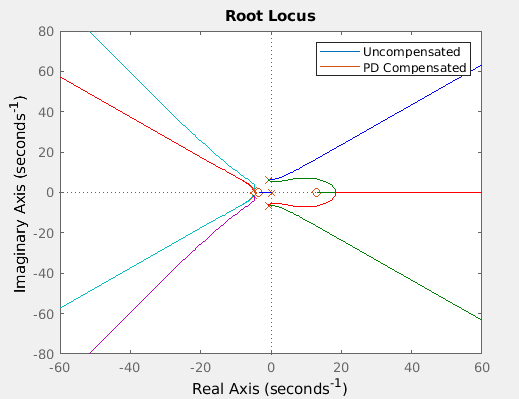
\includegraphics[width=\columnwidth]{lab6pidmatlabrl.png}
					\caption{Matlab Root Locus for $K_p = 0.38$, $K_i = 1.87$ and $K_d = -0.04$}
					\label{fig:lab6pidmatlabrl}
				\end{figure}
			\subsubsection{Ziegler-Nichols}
				The previous tuning done in \Cref{sec:pidtune} tuned based off of educated guesses of good starting points. And it worked, it was possible to get a very well tuned system. However, there are other, more empirical methods for tuning, one of which is the Ziegler-Nichols method \cite{elprocus}.
				\par
				\begin{table}
					
					\centering
					\begin{tabular}{l|l|l|l}
						& $K_c $ & $T_i$ & $T_d$ \\
						\hline
						PID & $\frac{K_u}{1.7}$ & $\frac{P_u}{2}$ & $\frac{P_u}{8}$\\
						\hline
						System Values & $0.741$ & $0.3475$ & $0.093625$\\
						\hline
					\end{tabular}
					\caption{Ziegler-Nichols Table \cite{elprocus}, with 
					filled out values}
					\label{tab:zn}
				\end{table}

				Using the simulink system, the ultimate gain is found to be $K_u = 1.26$ and the ultimate period is found to be $P_u = 0.749$. With these two values, the Ziegler-Nichols table can be used to find the values $K_c$, $T_i$ and $T_d$(\Cref{tab:zn}). These values result in PID values $K_p = K_c = 0.741$, $K_i = \frac{1}{T_i} = 2.670$ and $K_d = T_d = 0.093625$. After rearranging the compensator to match the one on \cite{elprocus}, and plugging those values, the response in \Cref{fig:lab6ZN} can be seen and should be seen as much worse than the response arrived to before. It oscillates much more and a has worse overshoot and settling time. This method does not appear to work with the system used in this paper, possibly due to the limitations on the system blocks as they have limits imposed on the range they can swing.

				\begin{figure}[!ht]
					\centering
					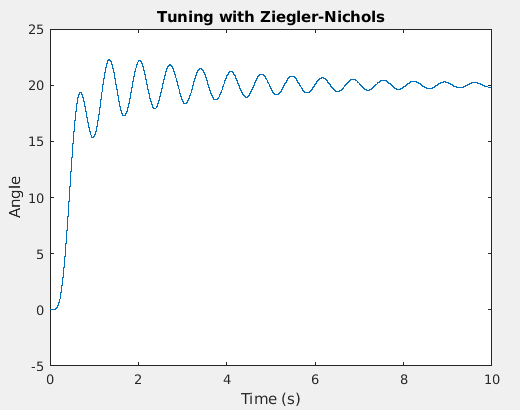
\includegraphics[width=\columnwidth]{lab6ZN.png}
					\caption{Ziegler-Nichols Step Response}
					\label{fig:lab6ZN}
				\end{figure}
	\section{Discussion}\label{sec:disc}
		So it is quite obvious that the system derived in the previous report is not the best representation of an actual system as evident by the variation in the step responses. However it has shown to be a good estimator for the system to allow educated guesses on where to start and when the system can be expected to go unstable.
		\par
		One of the components that has not shown heaps on improvement on the system is the D compensator. Positive $K_d$ values are what is expected, placing the zero in the stable region, so I'm not sure why this works out. Because by making it negative, this makes the whole equation negative, meaning the negative feedback is positive onto a negative equation.
		\par
		Another factor that would cause some disparity between the two models is that simulink implements the derivative component as $\frac{s}{cs+1}$ as it is unable to perform a non numeric derivative on something it doesn't have the equation for. This makes the simulink PD compensator actually a lead compensator which cuts off the infinite gain at high frequencies, something the matlab model has access to. This means that the matlab model would end up with more overshoot and oscillations for the same gain constants. Which is what is observed. 
		\par
		The kill switch implemented in \Cref{sec:p} isn't used in this report as everything is done via simulation. However, in a practical system it's use becomes more apparent. As mentioned in \Cref{sec:p}, when the system becomes unstable a flying fan is unideal as it poses a massive health and safety risk. This can happen from a few things such as gains that are too high, any value high enough will cause problems, and integral windup. Integral windup is a phenomenon that occurs when the system is unchanging while actively computing the integral, so the error continuously adds and the inputted voltage is going to be much higher. \Cref{fig:integralWindup} shows the simulation of this effect, but this rapid rise up and then oscillation around a high angle is also a risk to lab members. So the kill switch gives us the ability to turn it off if this happens.
		\begin{figure}[!ht]
			\centering
			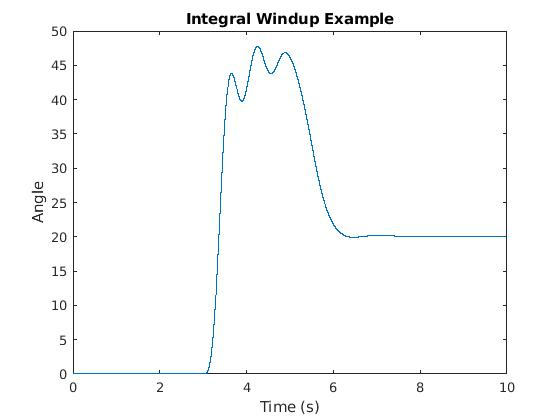
\includegraphics[width=\columnwidth]{integralWindup.jpg}
			\caption{Integral Wind up}
			\label{fig:integralWindup}
		\end{figure}
		\par
		The way that the PID compensator has been implemented follows \Cref{eq:pideq}, which makes the zero placement very dynamic as every value change will shift a zero. A better way to do it would be the way described in \cite{elprocus} and \Cref{eq:pideq2}. This method makes it so that only $K_i$ and $K_d$ have an influence on the zero placement and while $K_d$ does have an impact on the overall gain, the main gain tuning comes from $K_p$, making it possible to adjust this without fear of zero movement.
		\begin{equation}
			\label{eq:pideq2}
			\begin{split}
				K(s) & = K_p(1 + \frac{K_i}{s} + K_ds)\\
					 & = K_p\frac{K_ds^2 + s + K_i}{s}\\
					 & = K_pK_d\frac{s^2 +\frac{1}{K_d}s + \frac{K_i}{K_d}}{s}
			\end{split}
		\end{equation}
		\par

    \section{Conclusion}\label{sec:conc}
		This report has covered the tuning of a compensator for a practical model of a propeller driven pendulum. The results have then be compared to a previously derived mathematical model of the system and the differences in the responses discussed. Various compensators were explored in this report and eventually combined in a PID compensator. This removed most of the overshoot and almost all the oscillation while the settling time was reduced more than sixfold of the expected settling time, down to less than a second.
		\par
		A different, more empirical method was then trialed and found to be ineffective over using educated guesses found from the mathematical model. Beyond that, the discrepancies between the two systems were identified and discussed. 
		\par
		The next steps for this type of system is apply a PID compensator to a physical pendulum system and tune it using the same methods. From there, it should be possible to expand this model to other types of pendulums due to their similar nature, such as double or inverted pendulums. Alternative paths for this is program motion patterns for the systems so that they can move around smoothly, or to incorporate a form of human control.


    \Urlmuskip=0mu plus 1mu\relax
    \bibliography{bibliography}
    \bibliographystyle{IEEEtran}

    \onecolumn
	\appendices
		\crefalias{section}{appsec}
		\section{Lab 4 Calibration} \label{app:calibration}
			\begin{figure}[!ht]
				\centering
				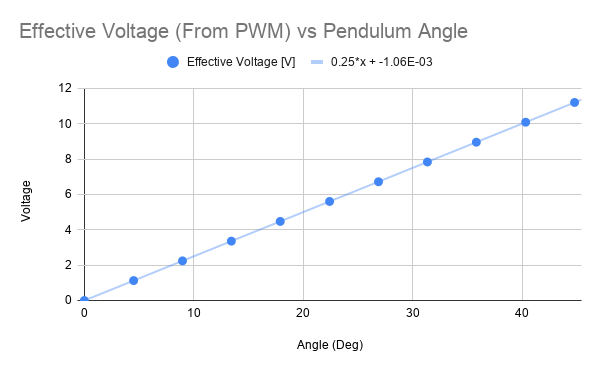
\includegraphics[width=0.8\columnwidth]{angleVoltage.png}
				\caption{Plot of Voltage applied to motor and the angular displacement produced}
				\label{fig:voltAngle}
			\end{figure}

			\begin{figure}[!ht]
				\centering
				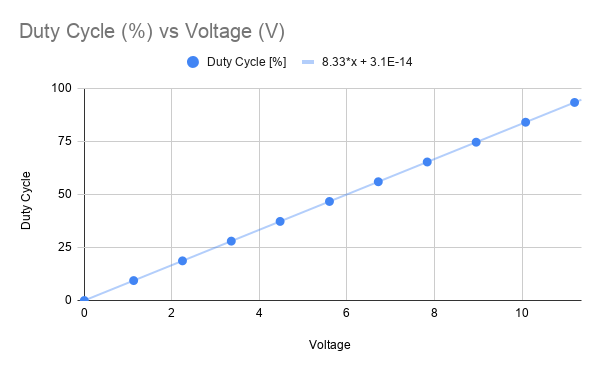
\includegraphics[width=0.8\columnwidth]{dutyCycleVoltage.png}
				\caption{Plot of effective voltage for a given duty cycle}
				\label{fig:DCV}
			\end{figure}

			\begin{figure}[!ht]
				\centering
				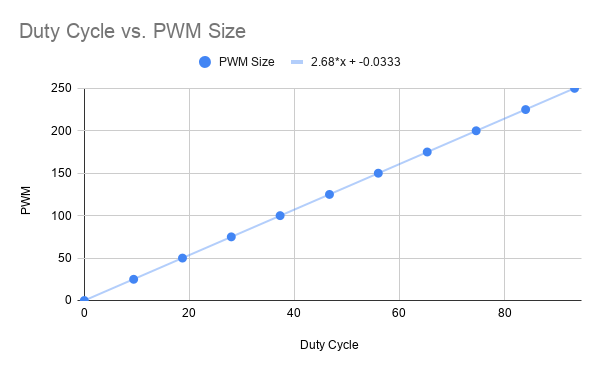
\includegraphics[width=0.8\columnwidth]{dutyCyclePWM.png}
				\caption{Plot of the Duty Cycle that a PWM value creates}
				\label{fig:DCPWM}
			\end{figure}

			\begin{figure}[!ht]
				\centering
				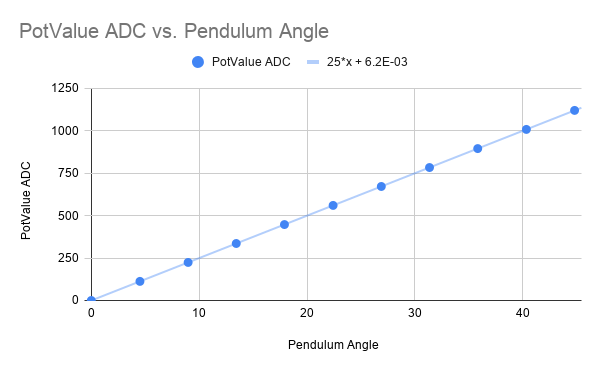
\includegraphics[width=0.8\columnwidth]{potPen.png}
				\caption{Plot of the potentiometer ADC value that an angular displacement causes.}
				\label{fig:potPen}
			\end{figure}
			
			\begin{figure}[!ht]
				\centering
				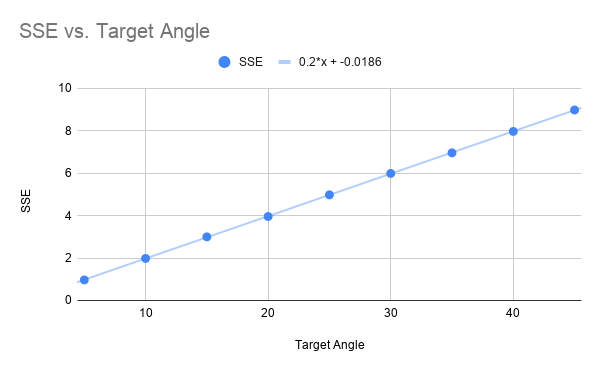
\includegraphics[width=0.8\columnwidth]{lab4SSEvsTarget Angle.png}
				\caption{SSE for a Given input angle when the system has error}
				\label{fig:lab4SSE}
			\end{figure}

		\section{Open Loop Transfer Function}\label{app:oltf}
			\begin{equation}
				\label{eq:systemDenom}
				\begin{aligned}
					V(s) = s^4 + \frac{ J_pJ_mR_a + J_pD_mL_a + J_mL_ac }{J_pJ_mL_a}s^3 + \frac{R_aD_mJ_p + K_tK_bJ_p + J_mR_ac + D_mL_ac + dmgJ_mL_a}{J_pJ_mL_a}s^2\\
					+ \frac{R_aD_mc + K_tK_bc + dmgJ_mR_a + dmgD_mL_a}{J_pJ_mL_a}s + \frac{dmgR_aD_m + dmgK_tK_b}{J_pJ_mL_a}\\
				\end{aligned}
			\end{equation}

			\begin{equation}
				\label{eq:fullTF}
				\begin{aligned}
					G(s) = \frac{\Theta(s)}{V(s)} = \frac{ \frac{K_tK_pr}{J_pJ_mL_a} }{ \cref{eq:systemDenom} }
				\end{aligned}
			\end{equation}
		\section{Closed Loop Transfer Function}\label{app:cltf}
			\begin{equation}
				a = \frac{ J_pJ_mR_a + J_pD_mL_a + J_mL_ac }{J_pJ_mL_a}
			\end{equation}
			\begin{equation}
				b = \frac{R_aD_mJ_p + K_tK_bJ_p + J_mR_ac + D_mL_ac + dmgJ_mL_a}{J_pJ_mL_a}
			\end{equation}
			\begin{equation}
				c =\frac{R_aD_mc + K_tK_bc + dmgJ_mR_a + dmgD_mL_a}{J_pJ_mL_a}
			\end{equation}
			\begin{equation}
				d = \frac{dmgR_aD_m + dmgK_tK_b}{J_pJ_mL_a}
			\end{equation}
			\begin{equation}
				\begin{split}
					T(s) & = \frac{K(s) \times \frac{ \frac{K_tK_pr}{J_pJ_mL_a} }{ s^4 + as^3 +bs^2 + cs + d }}{1 + K(s) \times \frac{ \frac{K_tK_pr}{J_pJ_mL_a} }{ s^4 + as^3 +bs^2 + cs + d }}\\
						 & = \frac{K(s) \times \frac{K_tK_pr}{J_pJ_mL_a}}{ s^4 + as^3 +bs^2 + cs + d + K(s) \times \frac{K_tK_pr}{J_pJ_mL_a}}
				\end{split}
			\end{equation}
\end{document}